\documentclass[12pt]{article}
% Set font to Times (similar to Times New Roman)
\usepackage[T1]{fontenc}
\usepackage{mathptmx}
% Set font size sections and subsections
\usepackage{sectsty}
\sectionfont{\fontsize{16}{15}\selectfont}
\subsectionfont{\fontsize{16}{15}\selectfont}
% Set document margins to 3cm
\usepackage[margin=3cm]{geometry}
\usepackage{cite}
\usepackage{amsmath,amssymb}
\usepackage{ctable}
\usepackage{tabularx}
\usepackage{float}
\usepackage[sc]{caption}
\usepackage{multirow}
\usepackage{microtype}
\usepackage{epstopdf}
\usepackage{verbatim}
\usepackage{verbatimbox}
\usepackage[multiple,bottom]{footmisc}
\usepackage[title,titletoc,toc]{appendix}
\usepackage{setspace}
\usepackage{rotating}
\usepackage{lscape}
%\usepackage{pdflscape}
\usepackage{subfigure}
\usepackage[para,online,flushleft]{threeparttable}
\usepackage{hyperref}
\usepackage{bm}
\usepackage{ragged2e}
\usepackage{epsf} 
\usepackage{graphicx}
\setlength{\parskip}{1em}
\setlength{\parindent}{0em}
% to allow capitalization of cross-references
\usepackage{cleveref}
\usepackage{bbold}
\usepackage[utf8]{inputenc}
\usepackage[english]{babel}
\setcounter{MaxMatrixCols}{20}
% Set footnote indent preferences
\makeatletter
\renewcommand\@makefntext[1]{\leftskip=0.5em\hskip0em\@makefnmark#1}
\makeatother
\addtolength{\footnotesep}{2mm}
% Set hyperlink looks
\hypersetup{colorlinks,urlcolor=blue,citecolor=black,linkcolor=black}
\makeatletter
\renewcommand*{\@cite@ofmt}{\bfseries\hbox}
\makeatother
\urlstyle{same}
%Para settings
\setlength\parindent{0pt}
\linespread{1.1}
% More enumaration formats
\usepackage{enumitem}
% More tabular formats
\newcommand{\specialcell}[3][c]{% 
\begin{tabular}[#1]{@{}#2@{}}#3\end{tabular}}
\usepackage{array}
\newcolumntype{P}[1]{>{\centering\arraybackslash}p{#1}}
% Biblio settings
\usepackage{natbib}
% Captions & Sources style
\usepackage[margin={1.5cm,1.5cm},labelfont=bf, font=small,justification=raggedright,singlelinecheck=false]{caption}
\newcommand{\source}[1]{\vspace{-3pt} \caption*{ Source: {#1}} }
% Set footnote size
\renewcommand{\footnotesize}{\small}

% Title, author, date
\author{Author: Ivan Vallejo Vall \\ Tutor: Iñigo Herguera García}
\title{%
  \vspace{-0.0cm}MASTER PROJECT \\ 
  \vspace{1cm} Measuring real broadband speeds using \\ crowdsourcing data from the Internet Foundation \\ \vspace{2cm} 
  }
\date{\vspace{1cm} Data Science Program 2016/2017 \\ 
\vspace{2cm} 
\includegraphics[scale=0.5]{Logo_GSE_green.png}}


\begin{document}
\linespread{1.4}\selectfont
\pagenumbering{gobble}% Remove page numbers (and reset to 1)
\maketitle
\newpage
\begin{abstract}
   Here goes the abstract-text, max 150 words.
\end{abstract}
\newpage
\tableofcontents
\newpage
\listoffigures
\listoftables
\newpage
\pagenumbering{arabic}% Arabic page numbers (and reset to 1)
\section{Introduction}
\subsection{Background}
The International Telecommunication Union -- ITU, the United Nations specialized agency for information and communication technologies (ICTs)\footnote{For more information on ITU, see \href{http://www.itu.int/en/about/Pages/default.aspx}{ITU's website}} -- is carrying out a series of pilot studies under the umbrella of the project Big Data for Measuring the Information Society (\autoref{fig:a1}).\footnote{For more information on the ITU project Big Data for Measuring the Information Society, see its \href{http://www.itu.int/en/ITU-D/Statistics/Pages/bigdata/default.aspx}{website}.} 
\vspace{1cm}
\begin{figure}[H]
    \centering
        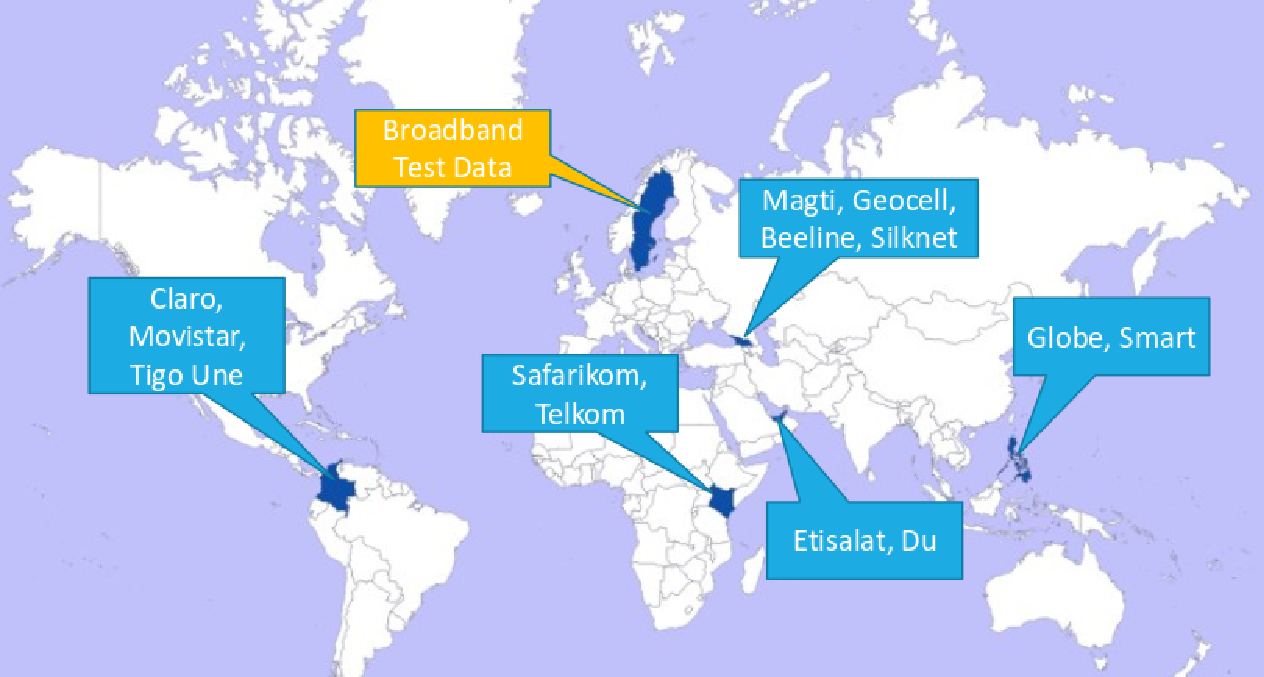
\includegraphics[width=\linewidth]{itu_projects.pdf}
        \caption{Big Data for Measuring the Information Society -- ITU pilot projects.}
        \caption*{\textbf{Source:} \cite{margus}.}
        \label{fig:a1}
\end{figure}   


The objective of the project is to show how big data from the telecommunication industry can be used to produce new ICT indicators and replace or complement existing ones with a view to measuring the development of the Information Society worldwide. 

In particular, these pilot studies aim to be a first step towards filling in the ICT data gaps in the global indicator framework agreed for the monitoring of the 2030 Agenda for Sustainable Development \citep{interagency}, and to inform private and public stakeholders on the current status of the digital divide.      

The object of this master thesis concerns the measurements on broadband speeds carried out by the Internet Foundation in Sweden (IIS)\footnote{The Internet Foundation in Sweden is an independent public-service organization which is responsible for the operation of the top-level domains '.se' and '.nu'. IIS reinvests part of the revenues obtained from the administration of these domains in activities to promote the stability of the Internet infrastructure in Sweden and research on the Internet. As part of these activities, IIS has developed the \textit{Bredbandskollen}, a software-based Internet platform to measure actual broadband speeds. For more information, see \href{https://www.iis.se/english/what-we-do/}{IIS website}} and made available to ITU in the context of the project Big Data for Measuring the Information Society.    

\subsection{Relevance}
Broadband speed measurements matter because they are a key input to several consumer, policy and regulatory decisions:

\begin{itemize}

	\item From a \textbf{consumer perspective}, broadband speed is one of the most important factors when choosing an Internet connection. For instance, in the European Union (EU) the download speed is the second most cited factor, after price, when deciding which broadband plan to choose.\footnote{On average, 41 per cent of respondents in the EU mentioned download speed as an important factor when subscribing to an Internet connection, compared with 71 per cent of respondents citing price. The figures refer to fieldwork carried out in January 2014.} However, six out of ten EU citizens do not know the maximum download speed of their broadband Internet plan and, among those that know it, a quarter of them believe that their real speed does not correspond to the one specified in their contract. Moreover, four in ten households in the EU admit having experienced difficulties accessing content at home because of speed or capacity issues \citep{eurobarometer}. It can thus be concluded that Internet speed is both an important and a controversial factor for consumers. 
	
	\item From a \textbf{regulatory perspective}, broadband speed is one of the parameters often monitored to ensure that telecommunication operators and Internet service providers (ISPs) comply with some minimum quality-of-service (QoS) requirements. For example, Spain regulates the QoS parameters of electronic communication services by means of a service order, which includes specific Internet access parameters \citep[Annex I, Part II in ][]{boe}. In a similar fashion, the Telecom Regulatory Authority of India sets that subscribers should get a minimum of 80 per cent of the speed specified in their contract, as measured from the ISP node to the user \citep{trai2006}.         
	
	\item From a \textbf{policy perspective}, broadband speeds have wide implications concerning the initiatives undertaken in the telecommunication sector. For instance, the definition of broadband is often tied to a given minimum speed, which is subject to be revised, as was the case in India in 2014 (from 256 to 512 kbit/s) \citep{trai2014}. In the United States, the Congress asked the Federal Communications Commission (FCC) to evaluate the deployment of \textit{advanced telecommunication capabilities}. FCC considered these capabilities to require 4 Mbit/s download and 1 Mbit/s upload speeds in 2010, but revised the benchmark speeds to 25 Mbit/s download and 3 Mbit/s upload in 2015 \citep{fcc2015a}. In Europe, Finland was a worldwide pioneer in declaring affordable broadband access a basic right in 2010. Finland's Ministry of Transport and Communications set the threshold for the basic connection to 1 Mbit/s in 2010, revising it to 2 Mbit/s in 2016 \citep{eprs}. All these policy decisions have deep economic implications. Indeed, in most cases they imply the mobilization of universal service funds (USF) or subsidy schemes to meet the targets set in terms of availability of affordable Internet connections at a given speed.        
\end{itemize}

In addition to these consumer, policy and regulatory implications, broadband speeds may also be an important determinant of broadband impact on economic growth \citep{bohlin2012}. Higher broadband speeds have also been found to be causally linked to increases in the percentage of employees classified as creative class workers \citep{whitacre2014}. 

All these factors motivate the interest in producing accurate data on actual broadband speeds.     

\subsection{Research questions}
\vspace{1cm}
\setlength{\fboxsep}{1em}
\centerline{\fbox{\begin{minipage}{0.8\linewidth}
\begin{enumerate}
\item Can crowdsourcing Internet data be used to measure real broadband speeds?
\item Which information can be extracted from online speed measurements to characterize Internet users?   
\end{enumerate}
\end{minipage}}}
\vspace{1cm}
Given the relevance of broadband speeds for consumers, regulators and policy-makers, there is a growing demand for accurate measurements. 

Advertised speeds, as publicized by operators and ISPs, provide only an upper-limit to the actual broadband speeds. On the other hand, precise external hardware-based measurements, such as the ones commissioned to SamKnows by the regulatory agencies in the UK \citep{ofcom2017}, the United States \citep{fcc2015b} and the European Commission \citep{samknows2013} are costly. Therefore, they cannot be realistically scaled up to a wider set of countries.  

Software-based, crowdsourcing data on Internet speed measurements remains the only possible stable source of real broadband speed information for most countries. Moreover, the low cost of deployment of these measurement platforms makes it possible to envisage its adoption by any interested regulator/policy-making. 

Indeed, some regulators in developing countries, such as the Telecommunications Regulatory Commission of Sri Lanka, have already launched their own measurement portal (\autoref{fig:a2}). Moreover, there are private stakeholders, such as Ookla, recording these data at the global level.\footnote{For more information on Ookla's Speedtest, see \Cref{meth} and \href{http://beta.speedtest.net/about}{Speedtest website}.} 

\begin{figure}[H]
    \centering
        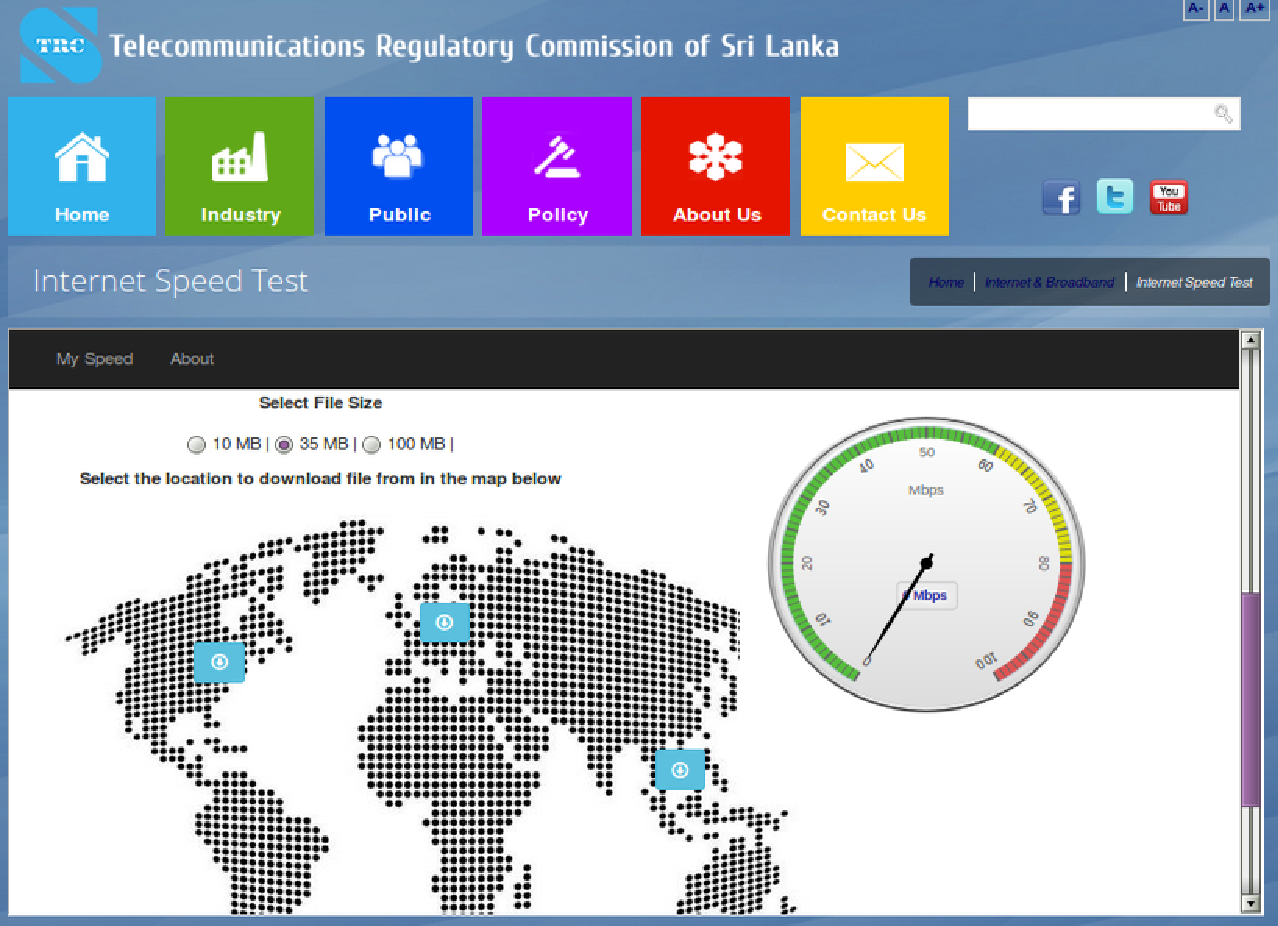
\includegraphics[width=\linewidth]{srilanka.pdf}
        \caption{Internet speed test platform,  Sri Lanka.}
        \caption*{\textbf{Source:} \href{http://www.trc.gov.lk/2014-05-12-13-25-54/internet-speed-test.html}{Telecommunications Regulatory Commission of Sri Lanka}.}
        \label{fig:a2}
\end{figure}   

In this context, the Internet Foundation in Sweden has been a forerunner of public-service broadband measurement platforms with its portal \textit{Bredbandskollen}, which collects data on Internet speeds since 2008 \citep{bredbandskollen}.   

This project takes advantage of the microdata made available by IIS to ITU on the broadband speed measurements from the \textit{Bredbandskollen} platform in the last six years (2011-2016). This large dataset is used as a testbed for determining to which extent this kind of crowdsourcing measurements can be used to provide robust insights into real broadband speeds, as well as information on Internet user behavior.  

\section{State of the art}
Broadband speeds are used by operators and ISPs as a means of characterizing their offers and segmenting their services according to different QoS. Advertised speeds are determined by each service provider according to their own internal methodology, which is not disclosed nor usually inspected by an independent party. However, it is understood that these speeds indicate the maximum or peak data rates that a customer may experience in the link between the customer location and the broadband provider \citep{bauer2010}.

More generally, advertised speeds are taken by customers to imply something meaningful about their experience when using a given broadband service. Since customers do not know in advance which Internet sites they will want to access, they demand universal connectivity from the ISPs and therefore expect advertised speeds to correspond to their end-to-end experience \citep[see the discussion on the MCI merger in][pp. 508-511]{economides2008}. 

For example, a customer contracting a 10 Mbit/s broadband plan with Movistar in Spain will expect to access information from The New York Times website at speeds close to 10 Mbit/s, even though the content of that website is hosted outside Movistar's network.      

Thus, the points from which to which the speed measurement is carried out matter for the consumer and explain part of the differences observed across different measurement platforms. \Cref{meth} reviews this and other technical factors having an impact on the state-of-the-art methodologies used to measure broadband speeds. \Cref{stats} presents how the problem of making statistical inference from crowdsourcing data on broadband measurements has been tackled in similar research efforts.   

\subsection{Measurement methodologies} \label{meth}

From a technical standpoint, the most accurate option for measuring real broadband speeds is to implement in-network measurements, such as real traffic monitoring (using network counters) or test-call routines. The technical issues concerning this type of measurements are well known. Indeed,  international standardization bodies, such as the European Telecommunications Standards Institute, have issued internationally agreed guidelines on how to perform this type of measurements \citep{etsi}.

In some countries, such as India and Spain, operators are required to self-report in-network measurements and the results are disclosed to the public on a regular basis \citep{setsi,zuhyle2015}.

However, in-network measurements can only be accomplished by those stakeholders having direct access to the network infrastructure and therefore rely on the self-reporting of the concerned network operators. Because of the difficulty of overseeing compliance and the lack of independence of this type of measurements, this approach is usually not considered a solution on its own, but rather a complement to other external measurements.

Therefore, external broadband speed measurements are the most common approach to gaining insights about real broadband speeds. There are a number of private stakeholders engaging in this kind of measurements and publishing data with a global coverage. These include, \textit{inter alia}, Ookla's Speedtest and Akamai speed reports \citep{bauer2010,lehr2013,bauer2016}. 

In addition, there exist several external broadband speed measurement platforms commissioned or operated by public entities and the academia. Some of them rely on hardware-based approaches, such as the SamKnows' Whitebox \citep{samknows2012,samknows2013} or the BISmark project's NoxBox \citep{sundaresan2012,sundaresan2014}. However, the majority of external measurements rely on purely software approaches. 

Examples of software-based approaches from public entities include the Regulatory Commission of Sri Lanka's Internet speed test platform \citep{zuhyle2015}, the Internet Foundation in Sweden's \textit{Bredbandskollen} and the Italian Authority for Communications Guarantees' \textit{Misurainternet} platform.\footnote{For more information, see the \href{https://www.misurainternet.it/}{Misurainternet website}}

These platforms collect several broadband performance metrics beyond download speed, such as upload speeds and latency (delay). Depending on the type of online activity performed, some parameters will be more important than others. For instance, latency is very relevant for real-time communications, such as VoIP. As a result of the diversity of activities performed online, a complete assessment of user quality of experience cannot be summarized into a single speed metric, but will require several complementary measurements \citep{samknows2013,zuhyle2015}. 

Moreover, there exist some application-specific broadband measurements, such as Netflix's Fast.com and Youtube's Speed numbers. These measurement platforms are optimized to reflect what is the actual speed experienced by a user transferring video files with the size and protocols common in Netflix and YouTube, respectively. However, these speed measurements may be a poor approximation of the actual speed experienced when browsing a website or sending a file \citep{bauer2010, bauer2016}.         

Based on a literature review of the state-of-the-art in broadband speed measurements, it can be concluded that external broadband speed measurement platforms depend on a few main design characteristics that affect their outcomes:

\begin{enumerate}[label=\textbf{\arabic* --}]
	\item \textbf{Measurement path:} from which point to which point of the network the measurement is made (\autoref{fig:a3}). Speeds advertised by operators refer to the maximum achievable over the access link (points 2-3 in \autoref{fig:a3}). In xDSL connections, the access link is not shared, as it is for coaxial cable, but xDSL speeds are more sensitive to the distance to the local exchange (path from 2 to 3). 
	
	From point 3 in \autoref{fig:a3}, there is contention for all wired technologies (fibre, coaxial, copper). That is, the transmission capacity is shared by many concurrent users and, depending on the network charge, this may lead to congestion and lower speeds. Even so, from points 2 to 4 the connection remains within the network of the ISP with whom the end user has contracted the service and therefore the speeds depend only on the network dimensioning and management of that ISP.
	
	End users' quality of experience is affected by the end-to-end path (i.e. points 1 to 5). This means that the speed experienced by a user also depends on the quality of the in-house connection (path from 1 to 2). For instance, the WiFi connection may not support high speeds or there might be several users making use of the same connection, therefore reducing the bandwidth available for the single user performing the test. Home network bottlenecks have been found to be very relevant in those settings in which the access is capable of providing speeds greater than 20 Mbit/s \citep{sundaresan2016}. 
	
\begin{figure}[H]
    \centering
        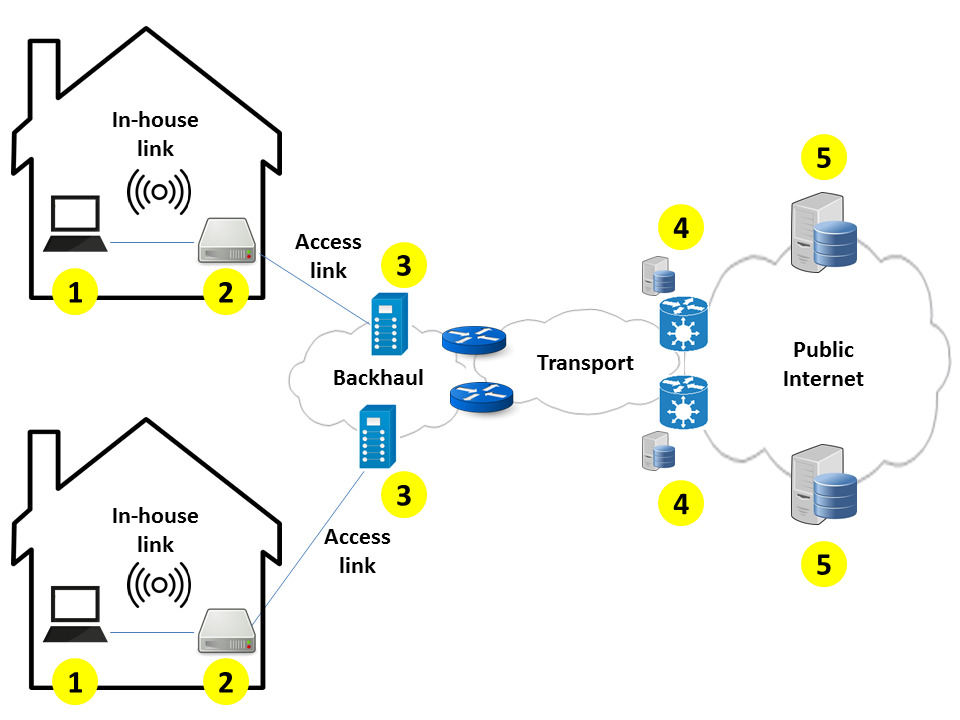
\includegraphics[width=\linewidth]{figure_network.png}
        \caption{Network diagram -- Key measurement points.}
        \caption*{\textbf{Source:} Author based on \cite{bauer2010}.}
        \label{fig:a3}
\end{figure}   
	
	In addition, end-to-end speeds may depend on other ISPs networks if the end user is accessing content hosted on the wider public Internet (off-net) instead of within the home ISP network (on-net). In the off-net case, the connection includes points 4 to 5 which are not under direct control of the home ISP. 
	
	However, it is the decision of the home ISP with whom to interconnect and under which conditions (e.g. traffic, peering). Therefore, under the assumption that customers demand universal connectivity from the ISP with whom they have the contract \citep[see][pp. 508-511]{economides2008}, this ISP could also be hold accountable for the speed delivered over the link from 4 to 5 in \autoref{fig:a3}. Indeed, ISP interconnection may have a substantial impact on consumer Internet performance and business relationships between ISPs are often at the root of this performance degradation, rather than technical issues \citep{m2014isp}.    

	\item \textbf{Active versus passive testing:} passive testing measures broadband speeds over end users' normal online activities, whereas active testing relies on standardized tests run independently of each end users' actual online activity. Active testing is usually preferred in benchmarking exercises because it facilitates the comparability between measurements \citep{zuhyle2015}. In passive testing, if two users are performing very different activities (e.g. heavy video streaming compared with light web browsing) the outcome of the speed measurements may be significantly different even if they have the same type of connection.

	\item \textbf{Voluntary versus automatic testing:} some broadband speed measurements are initiated by the end user (most software-based platforms, including Ookla and Bredbandskollen), whereas a few others are scheduled remotely and take place automatically (e.g. hardware-based platforms, such as SamKnows). Voluntary testing has several drawbacks, including the risk of selection bias. That is, end user's may run the test in a diagnostic fashion when they are experiencing network problems \citep{bauer2010}. Moreover, actual speeds are sensitive to congestion: they tend to decrease at peak hours or during traffic burst times \citep{sundaresan2012,zuhyle2015}. As a result, broadband speed results of voluntary tests may be biased because of the timing of the tests, which is out of control of the measurement platform and may not be randomly distributed. For instance, there could be more tests run during congestion periods because that is precisely when end users' perceive speed problems.          
	 
	\item \textbf{Data protocol configuration:} the data transmission protocol, usually TCP, may actually be the bottleneck if not correctly configured. This is more so in high-capacity networks (e.g. gigabit broadband networks), where a single TCP flow will most likely not be enough to measure the real capacity of the link. Therefore, multiple parallel TCP flows will be required to produce a reliable measurement in high-capacity networks \citep{bauer2010,bauer2016}.
	
	\item \textbf{Statistical aggregation:} results for individual tests are calculated using different methods. These include: (i) total bytes / total time, (ii) total bytes / total time after the ramp-up period, to exclude the initial warm-up period in which transmission is slower, and (iii) payload / bytes, so that only the actual information (and not the header aggregated by the transfer protocol) is considered. In addition, different aggregation methods are used for reporting aggregate statistics. For instance, SamKnows discards the top and bottom percentiles to control for outliers and averages the rest \citep{samknows2013}. Ookla removes the fastest 10 per cent and slowest 30 per cent slices of each measurement and averages the rest \citep{bauer2010}. \textit{Bredbandskollen} takes the higher between the average speed of the whole measurement period (10s) or the average of the last 8s.\footnote{See \textit{Bredbandskollen} methodological \href{https://ensupport.bredbandskollen.se/support/solutions/articles/1000228167-how-does-the-measurement-work-in-technical-terms-}{FAQ}.}   
	
	\item \textbf{Other design parameters}, such as test duration time, technology used in the application (e.g. HTML or Flash-based) and the file size used in download/upload measurements \citep{bauer2010,zuhyle2015}.             

\end{enumerate} 

\autoref{tab:t1} summarizes how this design parameters vary according to the broadband speed measurement platforms chosen in this project to benchmark the results obtained with \textit{Bredbandskollen}.

The main differences would be following: SamKnows ability to exclude the home network from the measurement and to automatically control the test timing, which will lead to more robust results; Akamai's passive testing, which may lead to comparing apples and oranges if their results are used to benchmark the outcome of active tests; the different statistical aggregation procedures which may potentially have a significant impact on the results.

Another relevant factor which needs to be considered is the different \textbf{sample sizes} of each broadband platform. For instance, concerning data from Sweden (i.e. the object of this project), \textit{Bredbandskollen} collected some 15 million observations per year for download speeds, Akamai 20 million and SamKnows 0.52 million. These differences illustrate the trade-off between volumes of data and precision of the measurement. Indeed, hardware-based measurements are costly and this severly limits the sample size even in developed countries.
\vspace{1cm}      
 
\begin{table}[H]
\bgroup
\def\arraystretch{1.5}%  1 is the default, change whatever you need
 \begin{tabular}{|p{3cm}|P{2.5cm}|P{1.6cm}|P{1.9cm}|P{2cm}|P{2.2cm}|}
  \hline 
   & \specialcell[c]{c}{\textbf{Measurement}\\ \textbf{path}} & \specialcell[c]{c}{\textbf{Active}\\\textbf{passive}} & \specialcell[c]{c}{\textbf{Voluntary}\\\textbf{automatic}} & \textbf{Data flows} & \specialcell[c]{c}{\textbf{Statistical}\\\textbf{aggregation}} \\ 
  \hline 
  \textbf{Akamai} & \specialcell[c]{c}{1-4 or 1-5\\depending on\\server load} & Passive & \specialcell[c]{c}{Real\\traffic} & Sequential & Unknown \\ 
  \hline 
  \textbf{Bredbandskollen} & \specialcell[c]{c}{1-4\\for most \\inland\\measurements} & Active & Voluntary & Parallel & \specialcell[c]{c}{Avg.first 2s\\or avg 10s} \\ 
  \hline 
  \textbf{Ookla} & \specialcell[c]{c}{1-4 or 1-5\\depending on\\user location} & Active & Voluntary & Parallel & \specialcell[c]{c}{Avg. after\\ramp-up\\Excl. top\\10\% and\\bottom 30\%\\slices} \\ 
  \hline 
  \textbf{SamKnows} & 2-5 & Active & Automatic & Parallel &  \specialcell[c]{c}{Avg. after\\ramp-up\\Excl. top\\and bottom\\percentiles}\\ 
  \hline 
  \end{tabular}
\egroup
  \caption{Main differences between selected Internet measurement platforms.}
  \caption*{\textbf{Source:} Author based on \cite{bauer2010, bauer2016,samknows2013} and \href{https://ensupport.bredbandskollen.se/support/solutions/articles/1000228167-how-does-the-measurement-work-in-technical-terms-}{Bredbandskollen}.}
        \label{tab:t1}  
\end{table}
  

\subsection{Statistical approach} \label{stats}

\Cref{meth} has dealt with what traditional statisticians would consider measurement error. This section looks into the issues related to the statistical treatment of the data. In particular, it looks at how similar studies have dealt with the problem of extracting representative insights about the whole population (or, at least, the in-scope population) 
based on non-representative Internet data. 

That is, given the data provided by a given broadband measurement platform (\textit{Bredbandskollen} in this project), how can we make statistical inference of the whole population or, at least, about some segments of it? 

Official indicators on telecommunications/ICTs are divided into two categories according to the source of the data collection: administrative data, and household surveys or censuses. The methodologies for collecting harmonized and internationally comparable ICT data from these two data sources are well know. See for instance the ITU Handbook \citep{handbook} and the ITU Manual \citep{manual}, respectively for administrative and survey ICT data sources.   

Big data, such as the millions of records obtained from broadband measurement platforms, are often a middle ground between these two types of data sources (\autoref{fig:a4}). 

Despite the large new datasets that are becoming available, if a given data source does not include all the data for a given type of measurement (e.g. the real broadband speed of all connections according to a given measurement approach), then it cannot be treated statistically as administrative data records and requires some of the techniques usually applied to survey data, such as those concerning sampling \citep{bigdata}.

Official ICT statistics from household surveys are grounded on probability-based sample surveys and a frequentist statistical framework \citep{couper2013}. However, there is much more statistical uncertainty about the measurement in the data collected from broadband measurement platforms than in the programmed surveys undertaken by national statistical offices. 

%\vspace{1cm}
\begin{figure}[H]
    \centering
        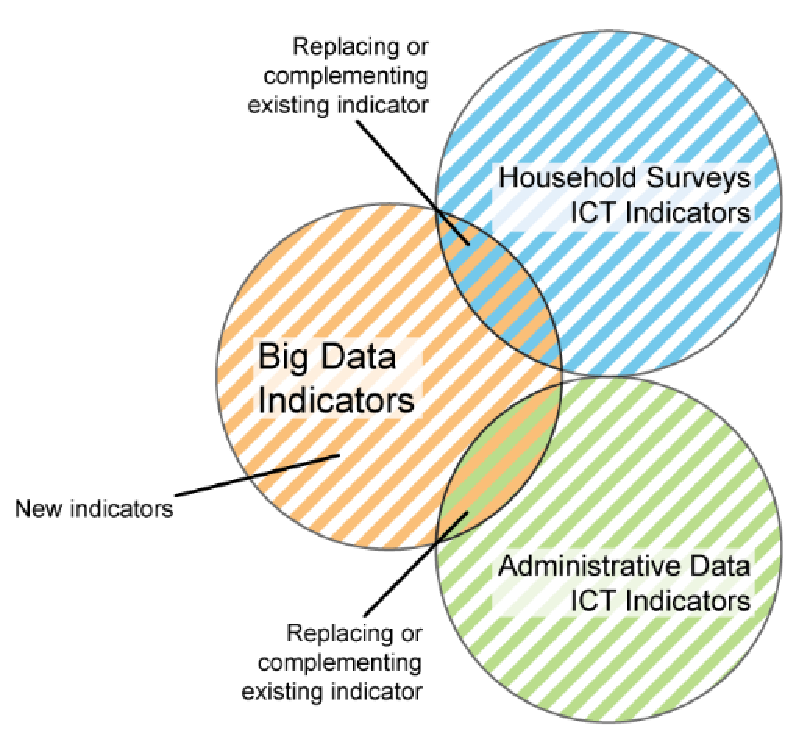
\includegraphics[width=0.5\linewidth]{admin_bd_hh.pdf}
        \caption{Data sources for official ICT statistics.}
        \caption*{\textbf{Source:} \cite{margus}.}
        \label{fig:a4}
\end{figure}   

Indeed, broadband speed measurements are composed of non-representative Internet data and, as such, face similar problems to those found in non-probabilistic samples \citep{couper2013,zagheni2015}:

\begin{enumerate}
	\item \textbf{Quota-based samples:} a panel is selected trying to make its composition proportional to the social, demographic and/or geographic characteristics of the in-scope population. More in general, quota-sampling is based on the selection of the surveyed individuals based on a series of covariates that are believed to explain the target variable. For instance, in its quota-based sampling methodology, SamKnows considers country, ISP and connection technologies to determine the quotas \citep{samknows2013}. Quota sampling in itself does not solve the issue of selection bias, particularly when participation is voluntary as in SamKnows studies.
	
	\item \textbf{Online voluntary surveys:} on top of the selection bias, unequal participation of the volunteers may add more uncertainty about the representativeness of the results. Indeed,  there is evidence from the survey research domain pointing that a relative large numbers of online surveys are completed by a relative small number of active panelists \citep{couper2013}. In the domain of broadband speed measurements, in some platforms where it is possible to identify individual end users, such in \textit{Bredbandskollen}, there is evidence that some active users ran thousands of tests per year, whereas some others only a few. In some other platforms, however, one-time test users were found to be predominant \citep{wattegama2011}. 
\end{enumerate}
	
From all statistical issues, selection bias is the central one when trying to make statistical inferences from the data produced by a broadband test platform. For instance, \cite{opt2012} used official statistics on geography, technology, gender and age\footnote{Official statistics on geography, technology, gender and age in the Netherlands are produced via household surveys by Statistics Netherlands (CBS) and administrative regulatory filings of ISPs to the Dutch regulator OPTA.} to test whether self-selected measurements of a broadband speed platform (iPing) where representative of the whole population. The results rejected this hypothesis, and concluded that higher speed connections as well as males and persons aged 30-60 were overrepresented. Moreover, the paper found that the results of Ookla's and Samknows' broadband measurement platforms in the Netherlands also risked not being representative of the whole population.

Several approaches have been proposed to deal with selection bias:

\begin{enumerate}

	\item \textbf{Selection panel:} create a proper selection panel from which to draw detailed socio-economic household and individual data in addition to the broadband measurements. This selection panel can then be used to weight the results of the self-selected panel and produce representative results out of it \citep{opt2012}. This is indeed a reliable but costly option, because it requires the maintenance of a regular panel in addition to the upkeep of the speed measurement application.
	
	\item \textbf{Calibration against ground-truth data:} use data from a reliable source (i.e. the so called ground-truth data) to weight the results of the broadband speed test in order to ensure that the results of the two sources correspond for a period in which they overlap.  This correction relies on the assumption that there is a (potentially stochastic) structural relationship between the subgroup of the population included in the broadband speed test sample and those not included. Moreover, this relationship needs to hold in time \citep{zagheni2015}. \citep{couper2013} notes that there is a risk of in-sample overfitting and type I errors when calibrating large datasets.
	
	\item \textbf{Differences-in-differences approach:} when it is not possible to obtain a robust point in time estimation because the previous approaches do not apply, it may still be possible to obtain a sound indication of trends by applying a differences-in-differences approach \citep{zagheni2015}. For such an approach to be feasible, a control group needs to be identified and the bias between the control and the measurement group needs to be constant with time. In addition, analogous to calibration, a key assumption needed to validate this approach is that relative changes for the subgroups of the population included in the sample are indicative of trends in the general population.         

\end{enumerate}  

Based on these points, a key question that needs to be addressed when analyzing broadband speed measurements is how volunteers taking part in the test differ from non-volunteers. This is a common question to most non-probabilistic survey research \citep{couper2013}. 

In practical terms, the statistical issues highlighted in this section often cannot be addressed \textit{a posteriori}; that is, during the data processing stage where the available information is fixed. 

For instance, a common problem when analyzing software-based broadband speed tests is that the information on the number of unique users is not available or not disclosed to the researchers \citep{canadi2012}. This is also the case in the \textit{Bredbandskollen} microdata that IIS shared with ITU, which for privacy issues does not contain a unique identifier for each user, but rather for each test. The lack of this information makes it difficult to perform any ex-post calibration, because the cross-linking of the observations from the speed measurement platform with external individual population characteristics is not possible.

When facing major problems inherent to the structure of the underlying dataset, researchers often follow the approach of describing the limitations of the dataset and publishing the results as such, with little \citep{prasad2016,wattegama2011,chetty2013} or some admonition about their representativeness for the whole population \citep{canadi2012,riddlesden2014}. In the latter, an approximate correspondence between the global average speed obtained in the study and that obtained in some previous more robust measurement effort is considered as a broad indication of the validity of the results.   
   
More generally, the validity of the statistical inference derived from each broadband speed measurement platform may depend on the purpose of the research. If the objective is to raise awareness that some consumers are getting real broadband speeds very different from the ones advertised in their contracts, showing that this is true for a large enough number of end users' may suffice \citep{chetty2013,wattegama2011}. 

If the purpose of a broadband speed measurement platform is customer self-check, a sound measurement methodology (as discussed in \Cref{meth}) and consistency in the results for a single user is all that is required. This is, for instance, the primary objective of Ookla's Speedtest. The Italian Authority for Communications Guarantees' \textit{Misurainternet} platform incorporates this logic in the application itself. Indeed, by means of an electronic certificate, legally validated results of the speed test can be communicated to the concerned ISP who then has the obligation to reestablish a minimum speed according to the conditions specified in the contract.

If the objective of the research is to obtain representative information on the real broadband speeds experienced by broadband subscribers in a country, as it is the case in official telecommunication statistics, then all the statistical considerations discussed in this section should be addressed.

Lastly, broadband speed measurement tests can also be a rich source of data for analyzing different Internet conditions and user behaviors across socio-economic strata. 

UK geolocation               
OPTA voluntary customer information  

\section{Data}
Bla bla
\subsection{Processing environment}
Bla bla
\section{Results}
Bla bla
\section{Conclusion}
Bla bla

%\nocite{*}

\bibliography{references}
\bibliographystyle{apalike}


\end{document}